\documentclass{C://Aliases//Dropbox-MIT//Latex_Templates//personal}

\author{Jack Dinsmore}
\title{GCE UROP Summary}

\begin{document}
\maketitle

\begin{abstract}
This month, I experimented with two luminosity functions: a power-law distribution, and a log-normal distribution. Each luminosity function has two free parameters which can be refined to match two recently-published observations made by the \textit{Fermi} space telescope.
\end{abstract}


\section{Introduction}
\subsection{The GCE}
The Galactic Center GeV Excess (GCE) is an unexpected source of gamma radiation originating from the center of the Milky Way, detected  recently by the \textit{Fermi} Gamma-ray Space Telescope \cite{fermilab}. Its origin is debated; the GCE holds potential to be the first evidence observed for dark matter annihilation, yet several studies have also shown that point sources such as millisecond pulsars (MSPs) may be responsible for the excess.

This UROP seeks to better understand the MSP model to the GCE by proposing different luminosity functions and counting the number of MSPs required to reproduce the GCE for each model, restricting the range of possibilities via \textit{Fermi}'s observations.

For the purposes of this summary, we will take the luminosity of the GCE to be \SI{6.37}{\erg \per\second}, which is consistent with the luminosity used in ref. \cite{fermilab}.


\subsection{Observations}
The \textit{Fermi} Space Telescope has observed two features which we explore in this summary. We model the sensitivity of the telescope as a step function, with the telescope detecting no pulsars of luminosity below $L_{t} = \SI{e34}{\erg\per\second}$ and all the pulsars above it.

As documented in ref. \cite{fermilab}, \textit{Fermi} has observed 47 point sources that could be part of the GCE. It is therefore likely that $N_t$, the number of MSPs in the GCE that have luminosity greater than \textit{Fermi}'s sensitivity is less than or equal to $N_t$. For any luminosity function, this observation will therefore limit the parameter space of distributions.

The same team discovered that the amount of flux visible from the GCE above the threshold of \textit{Fermi} is about one quarter of that below the threshold. We denote this ratio $R$. Similarly, it is likely that the true value of this ratio is less than or equal to one quarter, which further limits the parameter space of luminosity functions.


\subsection{Luminosity functions}
A luminosity function is the distribution of the MSP population's luminosity, $\frac{dN}{dL}$. We explore two basic luminosity functions. The first is a power law with a hard cutoff, parameterized by the minimum and maximum luminosities of the population $L_{min}$ and $L_{max}$ respectively: 
$$\frac{dN}{dL} = L^{-\alpha}, \indent L\in [L_{min}, L_{max}]$$
which was used by ref. \cite{fermilab}. Here, $\alpha$ is a fixed value which was taken at about $1.95$ by ref. \cite{fermilab} to match their observations, but could be 1.2 to 1.5 for a more physically realistic luminosity function. We also used a variant of this luminosity function, which is called a power law with an exponential cutoff:
$$\frac{dN}{dL} = L^{-\alpha}\expp{\frac{L}{L_{max}}}, \indent L\in [L_{min}, \infty]$$

The second luminosity function is log-normal parameterized by the mode luminosity $L_0$ and the standard deviation in log-space around that peak $\sigma$: 
$$\frac{dN}{dL} = \frac{\log_{10}e}{\sigma \sqrt{2\pi} L}\expp{-\frac{\parens{\log_{10} L - \log_{10}L_0}^2}{2\sigma^2}}, \indent L\in [0, \infty]$$
which was used by ref. \cite{log-normal}.

Of these, the log-normal luminosity function is more physically relevant, but the power law is simpler. Both have been studied in detail by the papers cited, but the observations from \textit{Fermi} have not yet been applied to a log-normal luminosity function, so it is useful to compare the two in this light.

We will mostly use an exponential cutoff for the power law luminosity function in this summary. The two models differ in projected number of MSPs in the GCE by only about 10 percent for values of $L_{min}$ and $L_{max}$ not to close to $L_t$, and increases to as much as 40 percent when $L_{min}, L_{max} \rightarrow L_t$.



\section{Power law luminosity function data}
Assuming that the luminosity function of the GCE is well modeled as a power law, a good first approach is to simply plot the number of pulsars necessary to produce the entire GCE as a function of the two parameters $L_{min}$ and $L_{max}$ of the power law. We can express the number of pulsars $N_t$ above \textit{Fermi}'s threshold and the ratio of luminosity $R$ above and below the threshold as a function of the parameters of the luminosity function also, which gives us a one-parameter family of configurations that matches each observation. See figure \ref{contour-overlay-power-law}. 

\begin{figure}[h]
    \label{contour-overlay-power-law}
    \centering
    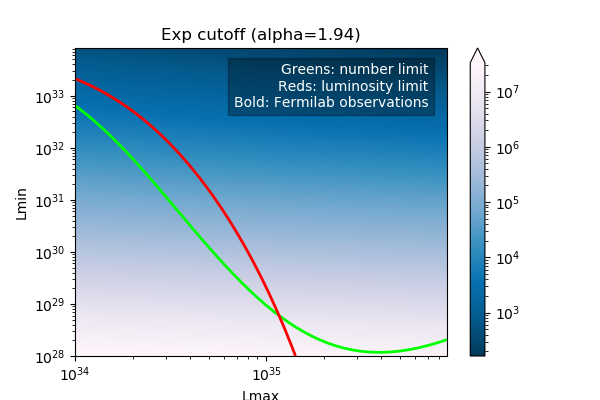
\includegraphics[width=0.6\textwidth]{../../luminosity-models/power-law/contour-overlay.png}
    \caption{Above is plotted the number of MSPs needed to reproduce the GCE under a power law luminosity with an exponential cutoff. In red is plotted the configurations required to match \textit{Fermi}'s observation of $R=1/4$, and in green their observation that $N_f = 47$. }
\end{figure}

The intersection point between these two families represents the only power law configuration that simultaneously realizes both of \textit{Fermi}'s observations, and it corresponds to $\si{3.3e6}$ MSPs in the GCE which is unrealistic. The region for $R < 1/4$ and $N_f < 47$, which is allowed by observation, appears beneath both curves.

To better understand this result, we show the same plot, but with contours representing other values of $R$ and $N_f$ superimposed on the number of pulsars (figure \ref{contour-overlay-extra-power-law}). One sees the limit imposed by the number of observed pulsars is more restrictive than that imposed by the luminosity observed above the threshold in this range of $L_{max}$.

\begin{figure}[h]
    \label{contour-overlay-extra-power-law}
    \centering
    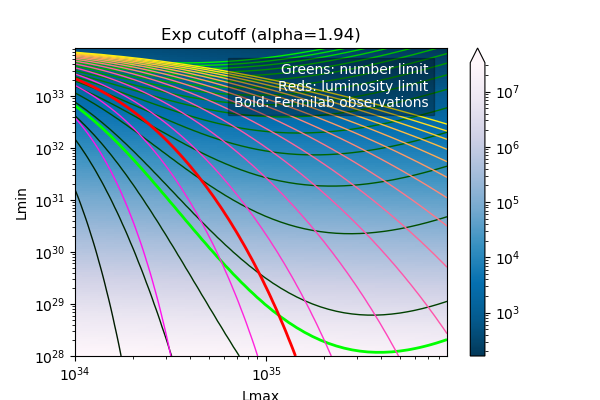
\includegraphics[width=0.6\textwidth]{../../luminosity-models/power-law/contour-overlay-extra.png}
    \caption{Above is plotted the number of MSPs needed to reproduce the GCE under a power law luminosity with an exponential cutoff. In red curves are plotted different values of $R$, with yellow representing higher values, while different values of $N_f$ are plotted in green, with brighter green representing higher $N_f$. The Fermilab results $R=1/4$ and $N_f=47$ are bolded.}
\end{figure}

To better understand the role of $\alpha$ in determining the intersection points of $R=1/4$ and $N_f = 47$, we can plot the curves representing these two families for many $\alpha$ (see figure \ref{contour-vary-alpha}). One can see that to satisfy both observational requirements, a high $L_{min}$ is required, quite close to $L_t$.

\begin{figure}[h]
    \label{contour-vary-alpha}
    \centering
    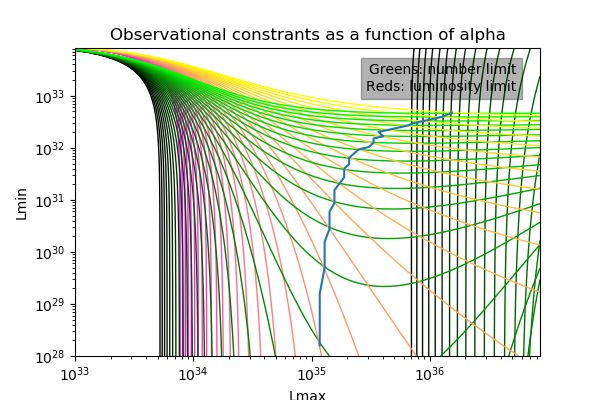
\includegraphics[width=0.6\textwidth]{../../luminosity-models/power-law/contour-vary-alpha-exp.png}
    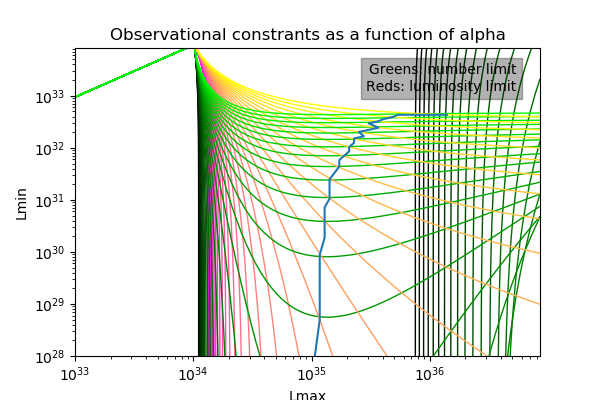
\includegraphics[width=0.6\textwidth]{../../luminosity-models/power-law/contour-vary-alpha-hard.png}
    \caption{Above is plotted the curves representing $R=1/4$ and $N_f=47$ for various $\alpha$ from 1.22 to 2.5. Higher $\alpha$ correspond to brighter colors. The blue curve represents the intersection points of these families for each $\alpha$. An exponential cutoff is used in the top plot, and a hard cutoff for the bottom.}
\end{figure}



\section{Log-normal luminosity function data}
For the sake of comparing a log-normal luminosity function to a power law, we can reproduce the same graphs for a log-normal luminosity function (figure \ref{contour-overlay-log-normal}). The region of $N_f \leq 47$ lies below the lower green line and above the upper, while $R \leq 1/4$ lies below the red line. Thus, the configurations allowed by \textit{Fermi}'s observations lies in the triangle below the lower green line. For these values of $R$ and $N_f$, the corresponding families are roughly parallel, but this is not true in general. From the lower plot in this figure, it can be seen that the curves in the upper plot do not vary greatly with changes in $R$ and $N_f$.

\begin{figure}[h]
    \label{contour-overlay-log-normal}
    \centering
    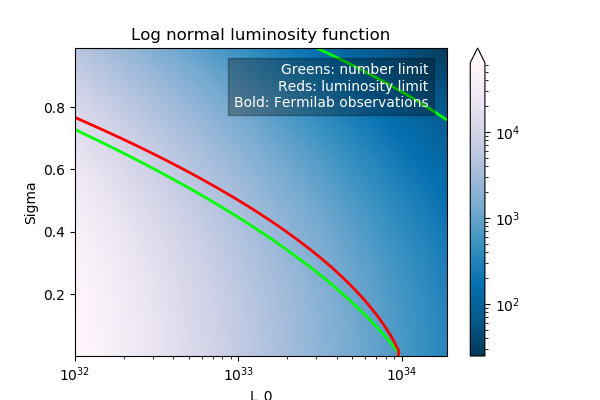
\includegraphics[width=0.6\textwidth]{../../luminosity-models/log-normal/contour-overlay.png}
    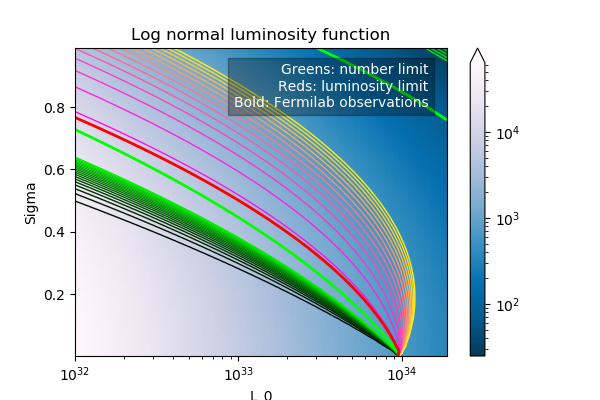
\includegraphics[width=0.6\textwidth]{../../luminosity-models/log-normal/contour-overlay-extra.png}
    \caption{The number of MSPs needed to reproduce the GCE under a log-normal luminosity. On the top plot, the configurations required to match \textit{Fermi}'s observation of $R=1/4$ are shown in red, and in green their observation that $N_f = 47$. The plot is expanded for the lower plot to different values of $R$ and $N_f$, with higher $R$ and $N_f$ represented by brighter colors.}
\end{figure}

The minimum number of MSPs inside this ``allowed triangle'' is 650, but that occurs for vanishingly low $\sigma$. Ref. \cite{log-normal} predicted values of $\sigma = 0.62^{+0.15}_{-0.5}$ and $L_0 = \brackets{0.88^{+0.79}_{-0.41}}\times\SI{e34}{\erg\per\second}$. Allowing $\sigma$ to range within one standard deviation of this assessment, the minimum number of pulsars required to reproduce the entire GCE and meet the $N_f=47$ requirement is $3920$, a reasonable number. This point occurs at $\sigma = 0.46$ and $L_0 = \SI{9.26e32}{\erg\per\second}$ and is shown as a blue dot in figure \ref{contour-overlay-log-normal}. However, the exact $(\sigma, L_0)$ components of the paper predict $N_f=121$ and $R=10$, which disagrees thoroughly with experiment.



\begin{thebibliography}{99}
    \bibitem{fermilab}Y. Zhong, S. McDermott, I. Cholis, P. Fox. ``A New Mask for An Old Suspect: Testing the Sensitivity of the Galactic Center Excess to the Point Source Mask.'' arXiv:1911.12369v (2019).

    \bibitem{log-normal}D. Hooper and T. Linden. ``The Gamma-Ray Pulsar Population of
    Globular Clusters: Implications for the
    GeV Excess.'' \textit{JCAP} (2016).

\end{thebibliography}


\end{document}